\chapter{Tests \& Results}

\section{Tests}
This section presents highlights from the testing suite of the pipelined MIPS processor with speculative execution. Branch prediction, data forwarding (including load-store forwarding), and pipeline flushing is demonstrated executing successfully.

\subsection{System integration test}

The provided system integration test from exercise 1,\todo{Add reference?}
which tests basic load, store, jump and arithmetic, was successfully run on the pipelined architecture.
The testbench has been extended to be more thorough, checking that the data from store
instructions following a branch taken doesn't end up in memory.

\subsection{Store after load operand forwarding}

The presented architecture has been extended to support operand forwarding from the write-back pipeline stage to the memory stage.
This allows for load instructions to be followed by store instructions without having to insert pipeline bubbles.

\begin{figure}[h]
  \begin{code}
    lui $3, 2
    srl $3, $3, 16   # Load 2 to $3
    lw $3, 1($0)     # Loads 1 from memory
    sw $3, 3($0)     # Should store 1, not 2 to address 3
  \end{code}
  \caption{Assembly to test store after load operand forwarding}
  \label{fig:test-store-after-load}
\end{figure}

Expected behavior:
\begin{itemize}
  \item
    The sw instruction should store the newly loaded value from the lw instruction, in effect acting like a memory move instruction.
  \item
    Bubbles should not be inserted into the pipeline.
\end{itemize}

\begin{figure}[ht!]
  \begin{center}
    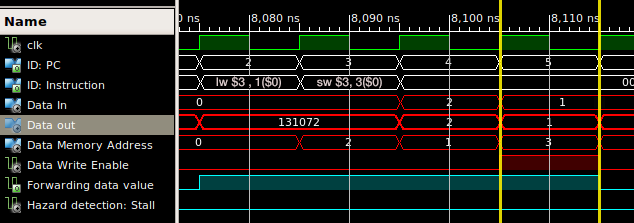
\includegraphics[width=\textwidth]{assets/lw-sw-forwarding.png}
  \end{center}
  \caption{Simulation of lw/sw forwarding}
  \label{fig:simulate_lw_sw}
\end{figure}

\subsection{Branch prediction}

The test case in figure \ref{fig:test-branch-prediction} tests both the hazard detection and branch prediction capabilities of the processor.

\begin{figure}[h]
  \begin{code}
    lw $1, 0($0)
    lw $2, 1($0)      # Should stall after this instruction (data hazard).
    beq $2, $0, 3     # Should predict (Control hazard).
    sw $2, 2($0)
    sub $2, $2, $1    # Introduce data hazard for beq
    j 2               # Jump to loop condition
    beq $0, $0, -1    # Loop forever
  \end{code}
  \caption{Assembly to test branch prediction} \label{fig:test-branch-prediction}
\end{figure}

Expected behavior:
\begin{itemize}
  \item
    The pipeline stalling on instruction 2. Branch after load requires one stall cycle to actually be able to correct for wrongly taken branches.
  \item
    The processor predicting whether instruction 2 should branch or not.
    Operands are available neither the first time (load not having completed yet), or after the end-of-loop jump (the sub instruction not having completed yet).
    As this architecture doesn't support operand forwarding to the branch predictor, it will have to guess.
\end{itemize}

\begin{figure}[h!]
  \begin{center}
    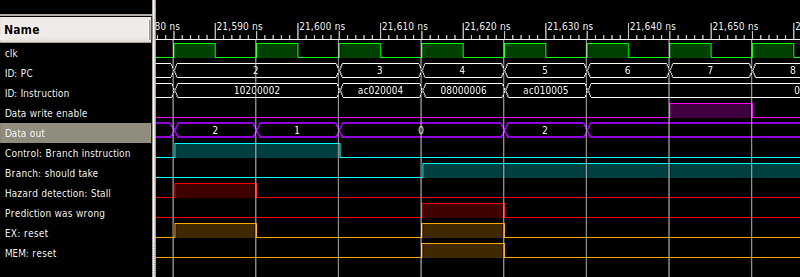
\includegraphics[width=\textwidth]{assets/pipeline-flushage.png}
  \end{center}
  \caption{Simulation of branch prediction}
  \label{fig:simulate_branch_prediction}
\end{figure}

\subsection{Pipeline flushing}

The test case in figure \ref{fig:test-pipeline-flushing} tests that speculatively executed instructions are correctly flushed from the pipeline.

\begin{figure}[h!]
  \begin{code}
    lw $2, 2($0)    # Loads 2 into $2
    lw $1, 1($0)    # Loads 0 into $1
    beq $1, $0, 2   # Branch speculatively not taken
    sw $2, 4($0)    # Speculatively executed, to be flushed
    j 6             # Speculatively executed, to be flushed
    sw $1, 5($0)    # Should actually be executed
  \end{code}
  \caption{Assembly to test pipeline flushing}
  \label{fig:test-pipeline-flushing}
\end{figure}

Expected behavior:
\begin{itemize}
  \item
    Instructions 3 and 4 should be speculatively executed, and flushed.
  \item
    Memory address 5 should have the value 2, address 4 should have the value 0.
\end{itemize}

\begin{figure}[ht!]
  \begin{center}
    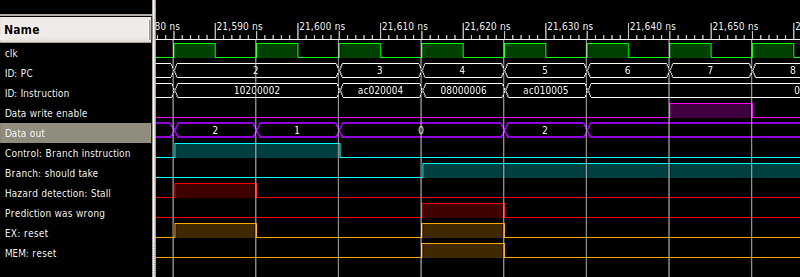
\includegraphics[width=\textwidth]{assets/pipeline-flushage.png}
  \end{center}
  \caption{Simulation of pipeline flushing}
  \label{fig:simulate_pipeline_flushing}
\end{figure}

\section{Component Tests}

\begin{table}[h]
    \begin{tabular}{|l|p{9cm}|l|}
    \hline
    \textbf{Unit under test} & \textbf{Test purpose}               & \textbf{Test status} \\ \hline
    PC                & Does the program counter increment normally? & \checkmark Passed \\ \cline{2-2}
                      & Can the program counter be paused? & \\ \cline{2-2}
                      & Is the correct order of overrides respected (branch predict, jump, branch correct)? & \\ \hline
    Forwarding unit   & Can data be forwarded from MEM stage to EX stage? & \checkmark Passed \\ \cline{2-2}
                      & Can data be forwarded from WB stage to EX stage? & \\ \cline{2-2}
                      & Can data be forwarded from WB stage to MEM stage? & \\ \cline{2-2}
                      & Is \$r0? ignored & \\ \cline{2-2}
                      & Will it incorrectly forward when control\_reg\_write is not enabled? & \\ \hline
    Two bit predictor & Confirm that the predictor defaults to 'not taken'. & \checkmark Passed \\ \cline{2-2}
                      & Check that two missed predictions are required before prediction switches. & \\\cline{2-2}
                      & Confirm that it properly resets to 'not taken'. & \\ \hline
    Hazard detection  & Confirm that the pipeline doesn't stall when an r-type instruction follows a load, but there's no overlap in registers & \checkmark Passed \\ \cline{2-2}
                      & Check that the pipeline stalls when a memory read precedes a dependent r-type or branch instruction. & \\\cline{2-2}
                      & Check that the pipeline doesn't stall when a data-dependent store instruction follows a load instruction. & \\ \hline
    Control unit      & Confirm that appropriate control signals are output for all supported instructions. & \checkmark Passed \\ \cline{2-2}
                      & Confirm that all outputs are zero when processor is not enabled. & \\ \hline
    \end{tabular}
    \caption{VHDL component tests}
    \label{fig:vhdl_component_tests}
\end{table}

\section{Results}

\subsection{Performance}
\todo{Throughput and clock frequency analysis compared to the multi-cycle design. Critical path and such}
\todo{Clock cycle comparison on system integration test, and the loop testbench}
\todo{Take inspiration from the previous report. Same tables and such}

\subsection{Power efficiency}
\todo{Power usage from isim}
